\documentclass[]{article}
\usepackage{lmodern}
\usepackage{amssymb,amsmath}
\usepackage{ifxetex,ifluatex}
\usepackage{fixltx2e} % provides \textsubscript
\ifnum 0\ifxetex 1\fi\ifluatex 1\fi=0 % if pdftex
  \usepackage[T1]{fontenc}
  \usepackage[utf8]{inputenc}
\else % if luatex or xelatex
  \ifxetex
    \usepackage{mathspec}
  \else
    \usepackage{fontspec}
  \fi
  \defaultfontfeatures{Ligatures=TeX,Scale=MatchLowercase}
\fi
% use upquote if available, for straight quotes in verbatim environments
\IfFileExists{upquote.sty}{\usepackage{upquote}}{}
% use microtype if available
\IfFileExists{microtype.sty}{%
\usepackage{microtype}
\UseMicrotypeSet[protrusion]{basicmath} % disable protrusion for tt fonts
}{}
\usepackage[margin=1in]{geometry}
\usepackage{hyperref}
\hypersetup{unicode=true,
            pdftitle={Response to Pachter's Review},
            pdfauthor={Joshua Paik and Igor Rivin},
            pdfborder={0 0 0},
            breaklinks=true}
\urlstyle{same}  % don't use monospace font for urls
\usepackage{color}
\usepackage{fancyvrb}
\newcommand{\VerbBar}{|}
\newcommand{\VERB}{\Verb[commandchars=\\\{\}]}
\DefineVerbatimEnvironment{Highlighting}{Verbatim}{commandchars=\\\{\}}
% Add ',fontsize=\small' for more characters per line
\usepackage{framed}
\definecolor{shadecolor}{RGB}{248,248,248}
\newenvironment{Shaded}{\begin{snugshade}}{\end{snugshade}}
\newcommand{\AlertTok}[1]{\textcolor[rgb]{0.94,0.16,0.16}{#1}}
\newcommand{\AnnotationTok}[1]{\textcolor[rgb]{0.56,0.35,0.01}{\textbf{\textit{#1}}}}
\newcommand{\AttributeTok}[1]{\textcolor[rgb]{0.77,0.63,0.00}{#1}}
\newcommand{\BaseNTok}[1]{\textcolor[rgb]{0.00,0.00,0.81}{#1}}
\newcommand{\BuiltInTok}[1]{#1}
\newcommand{\CharTok}[1]{\textcolor[rgb]{0.31,0.60,0.02}{#1}}
\newcommand{\CommentTok}[1]{\textcolor[rgb]{0.56,0.35,0.01}{\textit{#1}}}
\newcommand{\CommentVarTok}[1]{\textcolor[rgb]{0.56,0.35,0.01}{\textbf{\textit{#1}}}}
\newcommand{\ConstantTok}[1]{\textcolor[rgb]{0.00,0.00,0.00}{#1}}
\newcommand{\ControlFlowTok}[1]{\textcolor[rgb]{0.13,0.29,0.53}{\textbf{#1}}}
\newcommand{\DataTypeTok}[1]{\textcolor[rgb]{0.13,0.29,0.53}{#1}}
\newcommand{\DecValTok}[1]{\textcolor[rgb]{0.00,0.00,0.81}{#1}}
\newcommand{\DocumentationTok}[1]{\textcolor[rgb]{0.56,0.35,0.01}{\textbf{\textit{#1}}}}
\newcommand{\ErrorTok}[1]{\textcolor[rgb]{0.64,0.00,0.00}{\textbf{#1}}}
\newcommand{\ExtensionTok}[1]{#1}
\newcommand{\FloatTok}[1]{\textcolor[rgb]{0.00,0.00,0.81}{#1}}
\newcommand{\FunctionTok}[1]{\textcolor[rgb]{0.00,0.00,0.00}{#1}}
\newcommand{\ImportTok}[1]{#1}
\newcommand{\InformationTok}[1]{\textcolor[rgb]{0.56,0.35,0.01}{\textbf{\textit{#1}}}}
\newcommand{\KeywordTok}[1]{\textcolor[rgb]{0.13,0.29,0.53}{\textbf{#1}}}
\newcommand{\NormalTok}[1]{#1}
\newcommand{\OperatorTok}[1]{\textcolor[rgb]{0.81,0.36,0.00}{\textbf{#1}}}
\newcommand{\OtherTok}[1]{\textcolor[rgb]{0.56,0.35,0.01}{#1}}
\newcommand{\PreprocessorTok}[1]{\textcolor[rgb]{0.56,0.35,0.01}{\textit{#1}}}
\newcommand{\RegionMarkerTok}[1]{#1}
\newcommand{\SpecialCharTok}[1]{\textcolor[rgb]{0.00,0.00,0.00}{#1}}
\newcommand{\SpecialStringTok}[1]{\textcolor[rgb]{0.31,0.60,0.02}{#1}}
\newcommand{\StringTok}[1]{\textcolor[rgb]{0.31,0.60,0.02}{#1}}
\newcommand{\VariableTok}[1]{\textcolor[rgb]{0.00,0.00,0.00}{#1}}
\newcommand{\VerbatimStringTok}[1]{\textcolor[rgb]{0.31,0.60,0.02}{#1}}
\newcommand{\WarningTok}[1]{\textcolor[rgb]{0.56,0.35,0.01}{\textbf{\textit{#1}}}}
\usepackage{graphicx,grffile}
\makeatletter
\def\maxwidth{\ifdim\Gin@nat@width>\linewidth\linewidth\else\Gin@nat@width\fi}
\def\maxheight{\ifdim\Gin@nat@height>\textheight\textheight\else\Gin@nat@height\fi}
\makeatother
% Scale images if necessary, so that they will not overflow the page
% margins by default, and it is still possible to overwrite the defaults
% using explicit options in \includegraphics[width, height, ...]{}
\setkeys{Gin}{width=\maxwidth,height=\maxheight,keepaspectratio}
\IfFileExists{parskip.sty}{%
\usepackage{parskip}
}{% else
\setlength{\parindent}{0pt}
\setlength{\parskip}{6pt plus 2pt minus 1pt}
}
\setlength{\emergencystretch}{3em}  % prevent overfull lines
\providecommand{\tightlist}{%
  \setlength{\itemsep}{0pt}\setlength{\parskip}{0pt}}
\setcounter{secnumdepth}{0}
% Redefines (sub)paragraphs to behave more like sections
\ifx\paragraph\undefined\else
\let\oldparagraph\paragraph
\renewcommand{\paragraph}[1]{\oldparagraph{#1}\mbox{}}
\fi
\ifx\subparagraph\undefined\else
\let\oldsubparagraph\subparagraph
\renewcommand{\subparagraph}[1]{\oldsubparagraph{#1}\mbox{}}
\fi

%%% Use protect on footnotes to avoid problems with footnotes in titles
\let\rmarkdownfootnote\footnote%
\def\footnote{\protect\rmarkdownfootnote}

%%% Change title format to be more compact
\usepackage{titling}

% Create subtitle command for use in maketitle
\providecommand{\subtitle}[1]{
  \posttitle{
    \begin{center}\large#1\end{center}
    }
}

\setlength{\droptitle}{-2em}

  \title{Response to Pachter's Review}
    \pretitle{\vspace{\droptitle}\centering\huge}
  \posttitle{\par}
    \author{Joshua Paik and Igor Rivin}
    \preauthor{\centering\large\emph}
  \postauthor{\par}
      \predate{\centering\large\emph}
  \postdate{\par}
    \date{1/22/2020}


\begin{document}
\maketitle

{
\setcounter{tocdepth}{2}
\tableofcontents
}
\begin{quote}
\emph{``Academic politics are so vicious precisely because the stakes
are so small.''} - Henry Kissinger
\end{quote}

\begin{quote}
\emph{``The value of preprints is in their ability to accelerate
research via the rapid dissemination of methods and discoveries.''} -
\href{https://liorpachter.wordpress.com/2019/10/21/zero-data-rna-seq/}{Lior
Pachter}
\end{quote}

\hypertarget{introduction}{%
\subsection{Introduction}\label{introduction}}

Lior Pachter published a
\href{https://liorpachter.wordpress.com/2020/01/17/diversity-matters/}{review}
of our \href{https://arxiv.org/pdf/2001.00670.pdf}{paper} claiming that
age was the greatest contributor to the observed difference in citations
between signers of Letters A, B, and C. Any characterization of our
paper which says we do not account for age is \emph{false}. In this
response, we will clarify a few points in our paper, repeat the relevant
analyses, and show that citations per year is an age agnostic metric to
compare mathematicians. We will also go to some length to address
potential objections to this new analysis, and also show they are
categorically false. \textbf{To clarify, when comparing mean and median
citations per year amongst R1 Math Professors, A \textless{} B
\textless{} C.} This result still stands, as does the rest of our
analysis, post some revision to our data. Finally, we will clearly
demonstrate Professor Pachter's mistake, namely parameter tuning
(hypertuning) of his arbitrary age cutoff, to acheive a result which
supports his incorrect interpretation.

We appreciate Professor Pachter's review - it gives us a chance to make
our analysis stronger. We would note that a revision was already in the
works and that in a normal review process we would have had three months
to respond. However, as our character and ability as scientists were
attacked, we thought it was appropriate to reply as quickly as possible.

\hypertarget{corrections-and-clarifications}{%
\subsection{Corrections and
Clarifications}\label{corrections-and-clarifications}}

We would like to thank Lior for finding the bug in our appendix which
pushes the mean Google Scholar citations of B further away from A. We
agree that the sentence - ``while this is not optimal, a quick sample
size calculation shows that one needs 303 samples or 21\% of the data to
produce statistics at a 95\% confidence level and a 5\% confidence
interval.'' - is ridiculous.

We should explain exactly how the data collection took place. We used
the \href{https://pypi.org/project/scholarly/}{scholarly api} to
initially collect our Google Scholar citations data. But the issues were
that the scraper did not accurately differentiate between those who had
a generic name and the observed fact that older mathematicians (like
Cheeger or Gromov) do not have Google Scholar citations. To assure data
quality, we manually checked the google scholar citations of every
single letter signer, comparing publications when necessary.

However, the empirical difference in citations was staggering and we
could predict an objection. More professors from R2 (teaching focused
universities) signed A, so it could have pushed the average down. We had
already spent so much effort collecting Google Scholar citations, so we
made a choice to only collect MathSciNet data on R1 Math Professors,
which is why Professor Pachter did not have MathSciNet citations in our
dataset. This choice was not made explicitly enough in our first
version. Let us look at the NaN values of those who are full math
professors at R1 univesities.

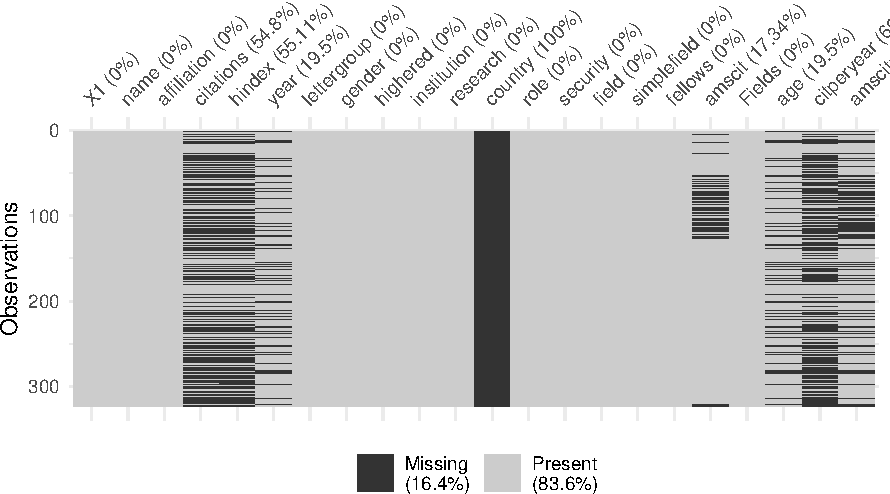
\includegraphics{index_files/figure-latex/unnamed-chunk-3-1.pdf}

One sees that 17.34\% of the Math Sci Net citations data is missing. It
appears there was some sort of systematic but unintentional error in the
data collection from MathSciNet. We report 3 NaNs on A and B, 3 on A
only, 0 on B and C, 50 on B Only, and 0 on C only. We manually checked
the missing data and find that all but
\href{https://www.math.arizona.edu/~civil/}{Marta Civil} and
\href{https://science.iupui.edu/people/watt-jeffrey}{Jeffrey X Watt}
(who are math educators) have Math Sci Net entries. The remaining
omissions are fixed and we visually check for NaNs again.

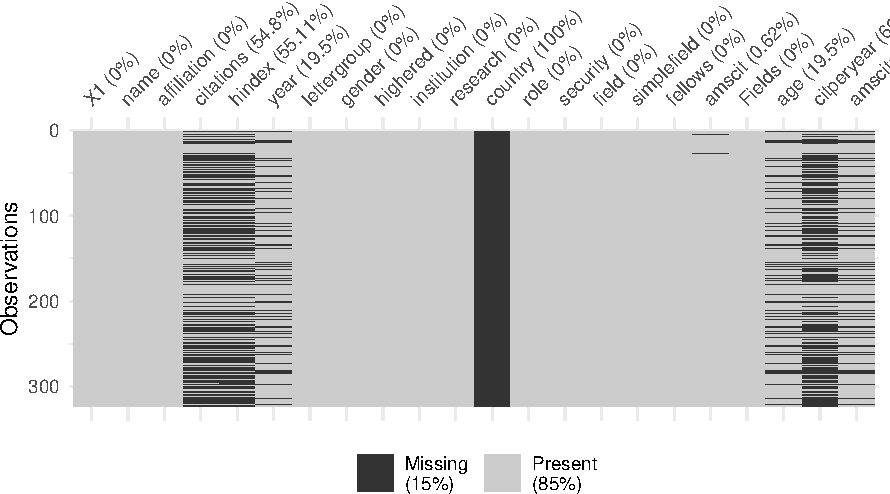
\includegraphics{index_files/figure-latex/unnamed-chunk-6-1.pdf}

65/323 is empty for AMS citations per year. While visually the nans
appear uniform, we will impose a stricter signifance level, say 2\%, to
assess the difference in AMS citations per year.

Now that we are comparing apples to apples, we reperform the main
results.

\hypertarget{the-main-result-of-paik-rivin-r1-math-professors-citations-and-citations-per-year}{%
\subsection{The Main Result of Paik-Rivin: R1 Math Professors Citations
and Citations per
Year}\label{the-main-result-of-paik-rivin-r1-math-professors-citations-and-citations-per-year}}

We will compare the mean number of citations and citations per year
between signers of Letters A, B, and C. We will validate the
significance of the difference between signers using a
\href{https://en.wikipedia.org/wiki/Resampling_(statistics)\#Permutation_tests}{permutation
test}.

The following is copy and pasted from our paper (with edit in
parentheses):

A permutation test is a nonparametric way of assessing the difference in
mean between two populations. We are interested in whether an observed
difference in mean is due to chance, and we can assess this in the
following way.

\begin{enumerate}
\def\labelenumi{\arabic{enumi}.}
\setcounter{enumi}{-1}
\tightlist
\item
  Record the true difference in mean (or median) (\(d\mu\)).
\item
  \(H_0: d\mu = 0, H_1: d\mu < 0\)
\item
  Sample without replacement 1/2 of the combined data set (X) and what
  is left (Y)
\item
  Take the mean (or median) of X and Y and record the difference
\item
  Repeat 10,000 times and plot the histogram
\item
  Record the number of points (m) in the induced distribution that is
  more extreme than or equal to the observed \(d\mu\). The probability
  m/10,000 is the probability that what was observed was due to chance.
\end{enumerate}

\hypertarget{mathscinet-citations-for-r1-math-professors}{%
\subsubsection{MathSciNet Citations for R1 Math
Professors}\label{mathscinet-citations-for-r1-math-professors}}

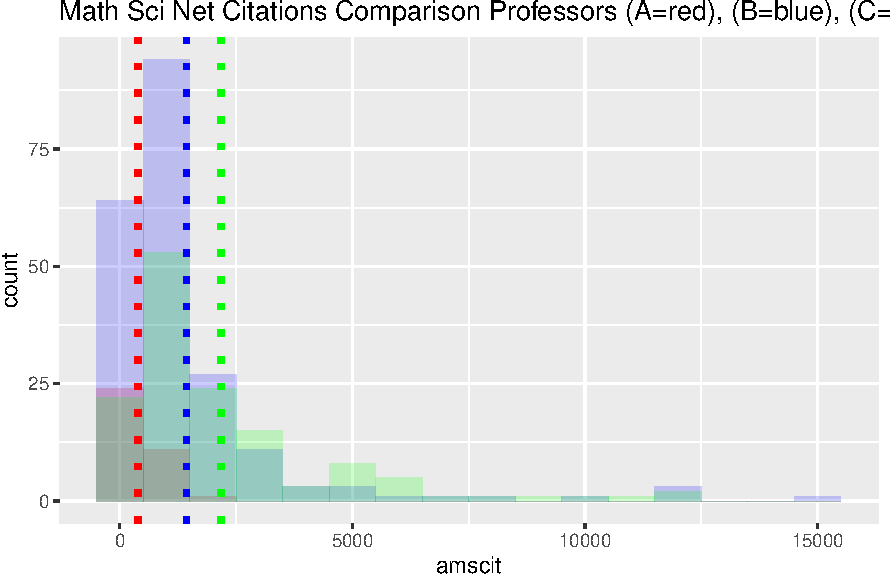
\includegraphics{index_files/figure-latex/unnamed-chunk-10-1.pdf}

The mean number of citations for signers of letter A is 397 and the
median is 261. The mean number of citations for signers of letter B is
1435 and the median is 915. The mean number of citations for signers of
letter C is 2177 and the median is 1353.

The three hypotheses we would like to assess are:

\begin{enumerate}
\def\labelenumi{\arabic{enumi}.}
\item
  \(H_0: \mu(A) = \mu(B), H_1: \mu(A) < \mu(B)\)
\item
  \(H_0: \mu(B) = \mu(C), H_1: \mu(B) < \mu(C)\)
\item
  \(H_0: \mu(A) = \mu(C), H_1: \mu(A) < \mu(C)\)
\end{enumerate}

In the following figure, the vertical red bar is the observed difference
for hypothesis 1 in the induced distribution, blue is the observed
difference for hypothesis 2, and green is the observed difference for
hypothesis 3.

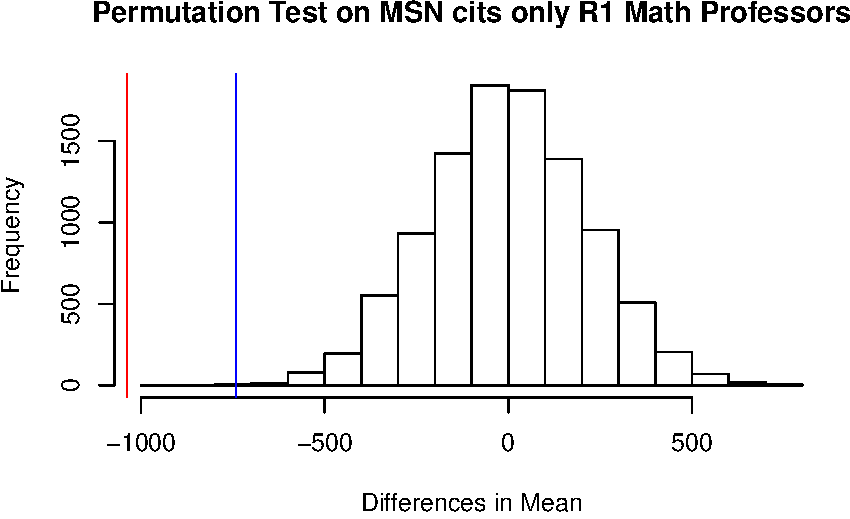
\includegraphics{index_files/figure-latex/unnamed-chunk-12-1.pdf}

The induced p-value for hypothesis 1 is 0. The induced p-value for
hypothesis 2 is 0.0002. The induced p-value for hypothesis 3 is 0. Hence
we reject all three null hypotheses in favor of the alternative, and
\(\mu(A) < \mu(B) < \mu(C)\).

\hypertarget{mathscinet-citations-per-year-for-r1-math-professors}{%
\subsubsection{MathSciNet Citations per Year for R1 Math
Professors}\label{mathscinet-citations-per-year-for-r1-math-professors}}

Of course, we considered the fact that citations grow with age, so we
calculated citations per year. There may be objections to this - one
could hypothesize that citations per year grow with age - but we will
soon thoroughly reject this claim.

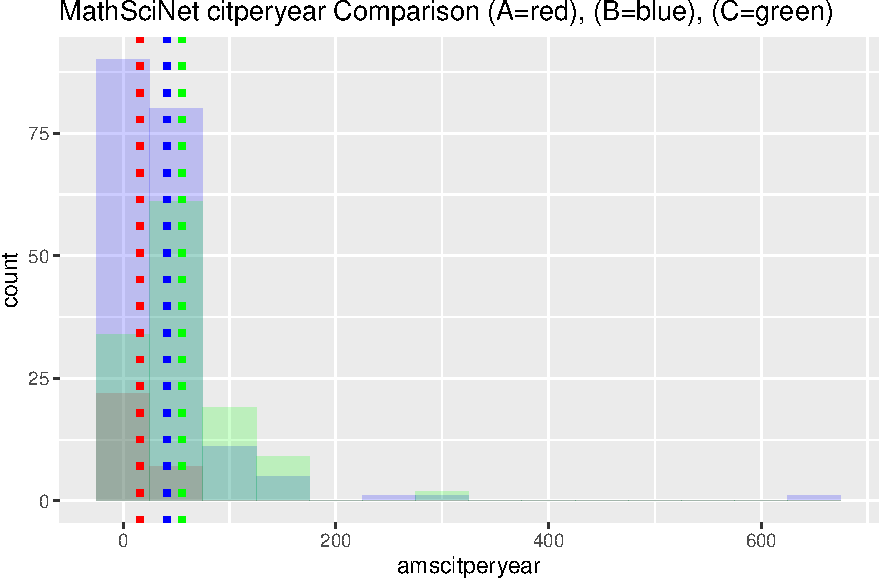
\includegraphics{index_files/figure-latex/unnamed-chunk-14-1.pdf}

The mean number of citations per year for signers of letter A is 16 and
the median is 11. The mean number of citations per year for signers of
letter B is 41 and the median is 26. The mean number of citations per
year for signers of letter C is 56 and the median is 42.

The three hypotheses we would like to assess are:

\begin{enumerate}
\def\labelenumi{\arabic{enumi}.}
\item
  \(H_0: \mu(A_{citperyear}) = \mu(B_{citperyear}), H_1: \mu(A_{citperyear}) < \mu(B_{citperyear})\)
\item
  \(H_0: \mu(B_{citperyear}) = \mu(C_{citperyear}), H_1: \mu(B_{citperyear}) < \mu(C_{citperyear})\)
\item
  \(H_0: \mu(A_{citperyear}) = \mu(C_{citperyear}), H_1: \mu(A_{citperyear}) < \mu(C_{citperyear})\)
\end{enumerate}

As above, the vertical red bar is the observed difference for hypothesis
1 in the induced distribution, blue is the observed difference for
hypothesis 2, and green is the observed difference for hypothesis 3.

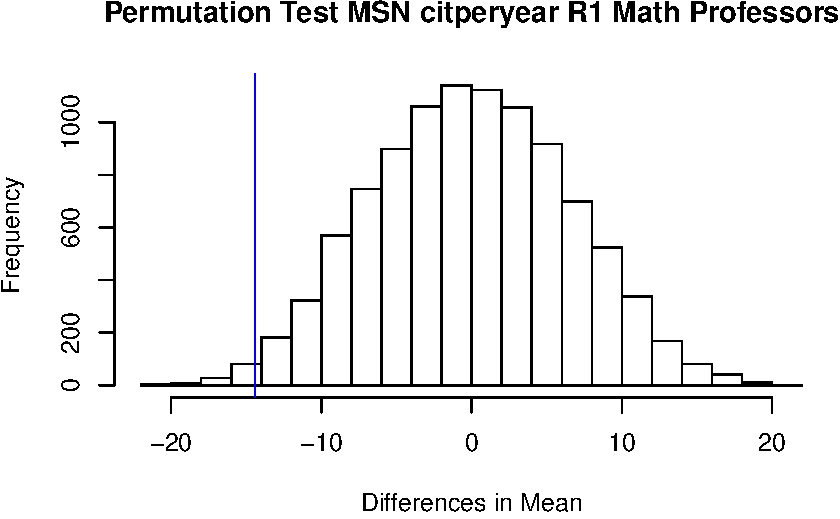
\includegraphics{index_files/figure-latex/unnamed-chunk-16-1.pdf}

The induced p-value for hypothesis 1 is 0. The induced p-value for
hypothesis 2 is 0.0099. The induced p-value for hypothesis 3 is 0. Hence
we reject all three null hypotheses, even assessing the induced p-value
at a 2\% significance level, in favor of the alternative, and we
conclude that
\(\mu(A_{citperyear}) < \mu(B_{citperyear}) < \mu(C_{citperyear})\).

One may object of our usage of the mean here, opposed to the median. So
we reperform the permutation test with the median. All three induced
p-values are 0 so we can reject all three null hypotheses when comparing
median citations per year.

\hypertarget{there-is-no-evidence-that-citations-per-year-grows-with-age}{%
\subsection{There is no evidence that Citations per Year grows with
age}\label{there-is-no-evidence-that-citations-per-year-grows-with-age}}

Let us check whether there is a relationship between age and citations
per year in our limited dataset.

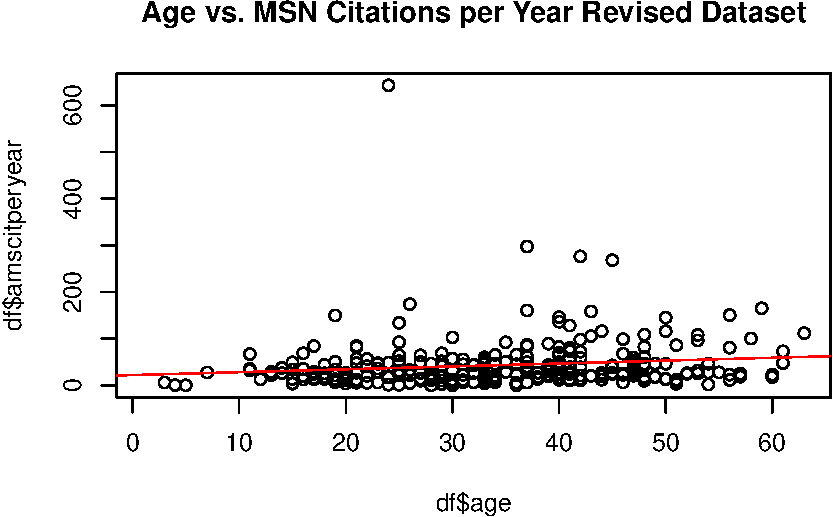
\includegraphics{index_files/figure-latex/unnamed-chunk-22-1.pdf}

\begin{Shaded}
\begin{Highlighting}[]
\KeywordTok{confint}\NormalTok{(linearmodel1)}
\end{Highlighting}
\end{Shaded}

\begin{verbatim}
##                 2.5 %    97.5 %
## (Intercept) 3.7459618 40.351608
## df$age      0.1149979  1.120528
\end{verbatim}

The slope of the regression line is slightly positive (0.6178, 95\%
Confidence Interval = (0.115, 1.12)), but the \(R^2\) values (Adjusted =
0.01662), are tragically low. So there is really no correlation. However
one could object that we do not have enough data (n = 258), to assess
that there is no correlation between citations per year and age. We know
this, but thought it would more appropriate to analyze this in a
separate paper. However, as noted above, our honor and ability as
scientists were attacked so\ldots{}

\hypertarget{presenting-citations-data-on-every-r1-math-professor-with-mathscinet-citations}{%
\subsubsection{Presenting citations data on every R1 Math Professor with
MathSciNet
citations}\label{presenting-citations-data-on-every-r1-math-professor-with-mathscinet-citations}}

(plus the Institute of Advanced Studies and UC Merced)

We manually collected the citations and year of first publication of
every R1 full math professor by consulting
\href{https://en.wikipedia.org/wiki/List_of_research_universities_in_the_United_States}{wikipedia},
going to the relevant faculty pages and then collecting MathSciNet
citations. We then anonymized it. The 2787 professors we collected data
on is in line with
\href{http://www.ams.org/profession/data/annual-survey/2016dp-tableDF1.pdf?fbclid=IwAR1mgI0qSEs5nCGquqye741_0lZU-ez7dlcJ3wZYhDtJUswhH1SX7yeiiak}{data}
collected by the AMS, after taking into account that about half of
universities in the US are classified R2. Great lengths were taken to
assess the accuracy of this data, including correlating publications,
PhD years, etc. Of course errors in data collection, especially manual
typing errors, happen, but by no means are these errors systematic.

\textbf{Exercise 1: Pick your favorite R1 institution, go to MathSciNet,
and check how similar our data is to what you determined.}

\textbf{Exercise 2: Determine every university without a female
professor. We will note that the University of Colorado - Denver has a
very strong female professor, but she does not have MathSciNet
citations. There should be at least one surprise (and a few non
surprises).}

Many aspects of this dataset can, should, and will be analyzed. For now,
the following will suffice.

\hypertarget{citations-per-year-vs-age}{%
\subsubsection{Citations per Year vs
Age}\label{citations-per-year-vs-age}}

We plot the Age vs Citations per Year for all math R1. We generate a
linear regression model and output a 95\% confidence interval for the
slope. 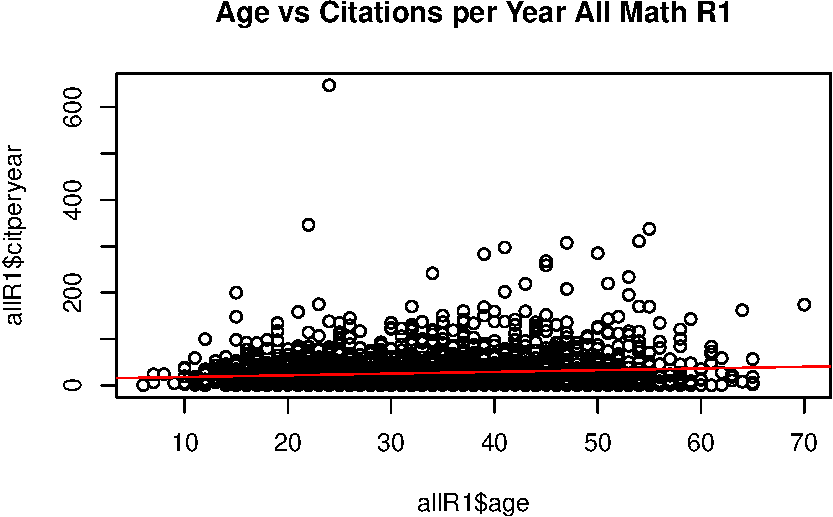
\includegraphics{index_files/figure-latex/unnamed-chunk-27-1.pdf}

\begin{Shaded}
\begin{Highlighting}[]
\KeywordTok{confint}\NormalTok{(linearmodel2)}
\end{Highlighting}
\end{Shaded}

\begin{verbatim}
##                  2.5 %   97.5 %
## (Intercept) 10.1588495 18.33147
## allR1$age    0.2515584  0.48675
\end{verbatim}

So while visually it appears that there is no correlation between
citations and citations per year, one may object and say, the slope is
positive! Which leads to the following question.

\textbf{Question: To what power must we raise age to get zero within the
confidence interval of slope.}

We object to this question, because the implication of the question is,
by how much should we discount the accomplishments of those who are
older. Nevertheless, we proceed.

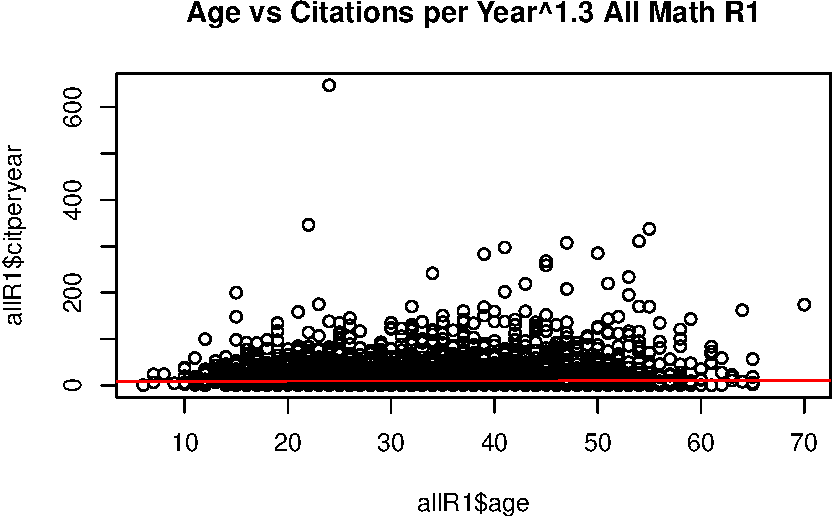
\includegraphics{index_files/figure-latex/unnamed-chunk-30-1.pdf}

\begin{Shaded}
\begin{Highlighting}[]
\KeywordTok{confint}\NormalTok{(linearmodel3)}
\end{Highlighting}
\end{Shaded}

\begin{verbatim}
##                    2.5 %     97.5 %
## (Intercept)  6.715962422 9.56734674
## allR1$age   -0.004656401 0.07740065
\end{verbatim}

It seems raising age to the 1.3 will do the trick.

We will reperform the permutation test comparing citations per
year\^{}1.3.

\hypertarget{citations-per-year-adjusting-for-fitted-handicap-on-age}{%
\subsubsection{Citations per Year adjusting for fitted handicap on
age}\label{citations-per-year-adjusting-for-fitted-handicap-on-age}}

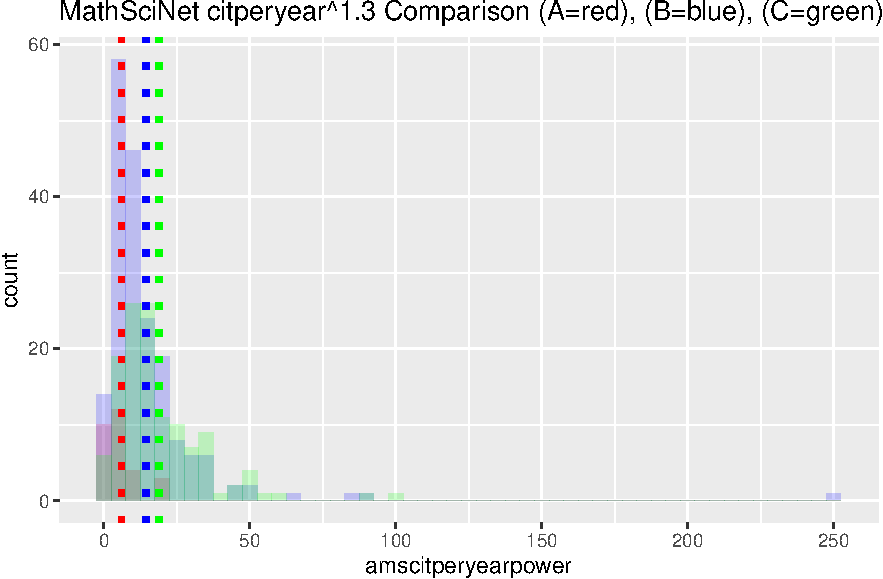
\includegraphics{index_files/figure-latex/unnamed-chunk-32-1.pdf}

The mean number of citations per year\^{}1.3 for signers of letter A is
6 and the median is 4. The mean number of citations per year\^{}1.3 for
signers of letter B is 14 and the median is 9. The mean number of
citations per year\^{}1.3 for signers of letter C is 19 and the median
is 14.

The three hypotheses we would like to assess are:

\begin{enumerate}
\def\labelenumi{\arabic{enumi}.}
\item
  \(H_0: \mu(A_{citperyear^{1.3}}) = \mu(B_{citperyear^{1.3}}), H_1: \mu(A_{citperyear^{1.3}}) < \mu(B_{citperyear^{1.3}})\)
\item
  \(H_0: \mu(B_{citperyear^{1.3}}) = \mu(C_{citperyear^{1.3}}), H_1: \mu(B_{citperyear^{1.3}}) < \mu(C_{citperyear^{1.3}})\)
\item
  \(H_0: \mu(A_{citperyear^{1.3}}) = \mu(C_{citperyear^{1.3}}), H_1: \mu(A_{citperyear^{1.3}}) < \mu(C_{citperyear^{1.3}})\)
\end{enumerate}

As above, the vertical red bar is the observed difference for hypothesis
1 in the induced distribution, blue is the observed difference for
hypothesis 2, and green is the observed difference for hypothesis 3.

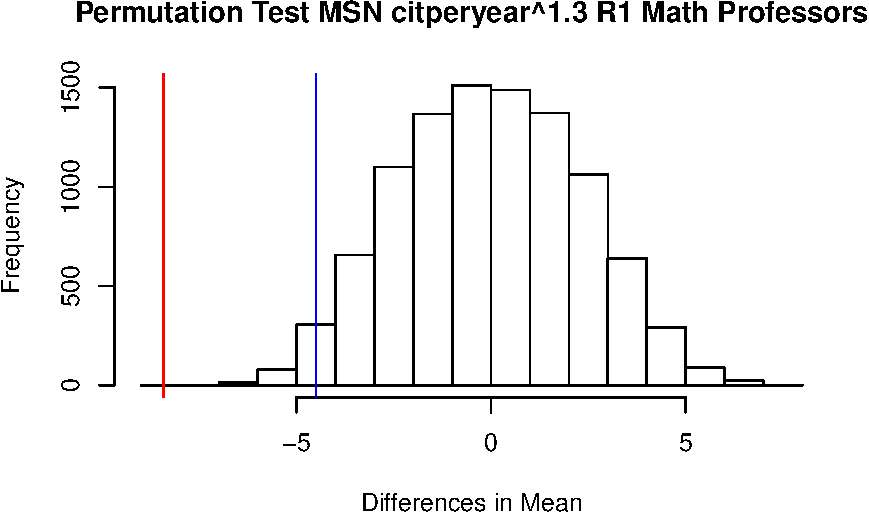
\includegraphics{index_files/figure-latex/unnamed-chunk-34-1.pdf}

The induced p-value for hypothesis 1 is 0. The induced p-value for
hypothesis 2 is 0.0207. The induced p-value for hypothesis 3 is 0. Hence
we fail to reject hypothesis 2 at a 2\% significance level and reject
hypotheses 1 and 3 in favor of the alternative. We conclude that after
adjusting for age \(\mu(A) < \mu(B) \leq \mu(C)\).

\hypertarget{one-more-check-that-age-is-irrelevant-when-comparing-citations}{%
\subsection{One more check that age is irrelevant when comparing
citations}\label{one-more-check-that-age-is-irrelevant-when-comparing-citations}}

This method was suggested by a friend as a final check to eliminate any
question that age was the greatest confounder. We want to show that
\(\mu(A) < \mu(B \cup C)\). We will randomly sample a population of 20
from A, called \(X\). For each member \(x \in X\), we will find every
person from B and C that is within a two year age interval from \(x\).
We will randomly sample one, and induce a new population \(Y\). Then we
will compare the means by storing X-Y. We repeat this 1,000 times and
plot a histogram of the induced values. If 0 is within this new
distribution, then maybe there is a chance, a totally slim one after
above, that in fact age is a confounder. If the distribution is
primarily negative, then X \textless{} Y. Otherwise X \textgreater{} Y.
We perform this analysis with both AMS citations and Google Scholar
citations.

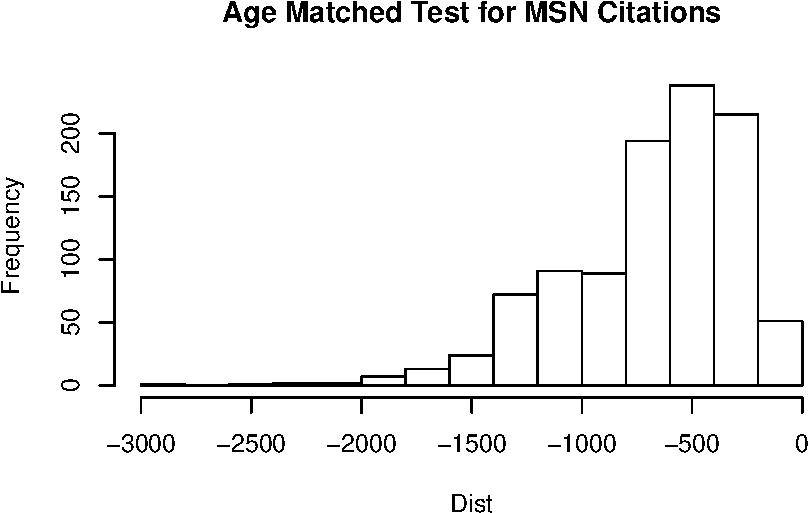
\includegraphics{index_files/figure-latex/unnamed-chunk-36-1.pdf}

When comparing mathscinet citations with this age matched randomization
test, we see that none of the induced distribution is greater than or
equal to zero. So when comparing similarly aged apples to apples,
\(A < B\cup C\)

We perform the same analysis with Google Scholar citations.

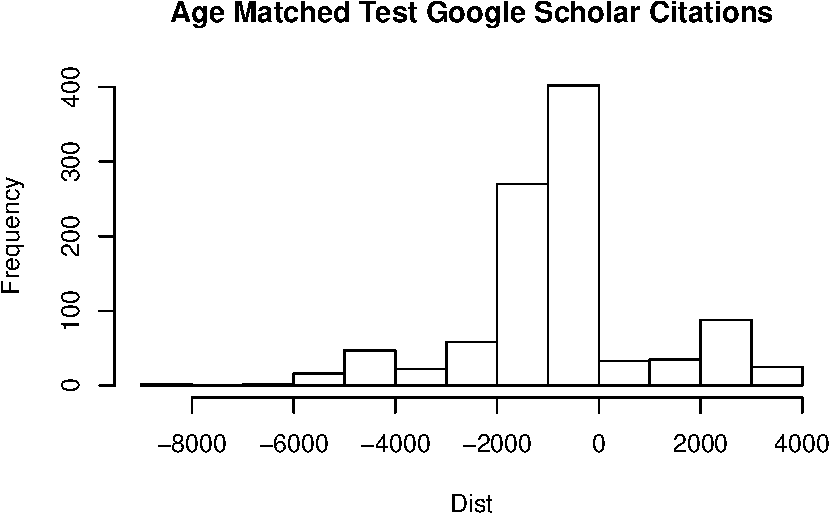
\includegraphics{index_files/figure-latex/unnamed-chunk-38-1.pdf}

When comparing Google Scholar citations with this age matched
randomization test, we see that 18.1\% of the induced distribution is
greater than or equal to zero. So when comparing similarly aged apples
to apples, it is inconclusive if \(A < B\cup C\). Of course, we wonder
if this is actually Lior Pachter.

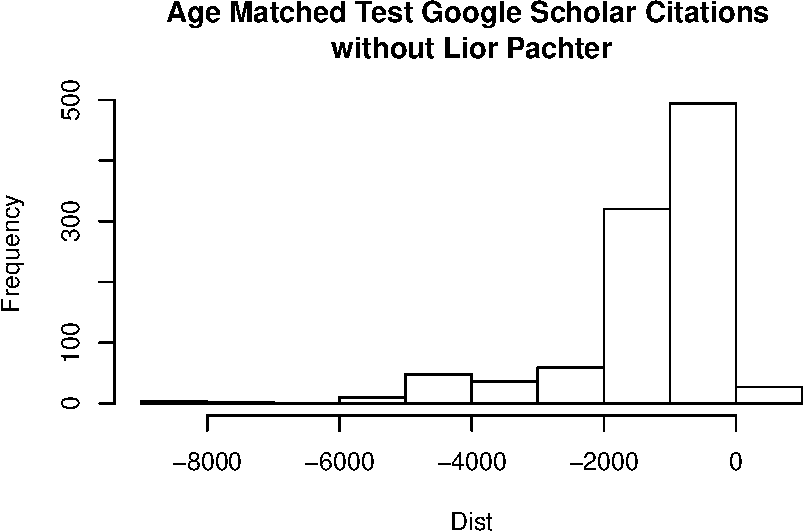
\includegraphics{index_files/figure-latex/unnamed-chunk-40-1.pdf}

When comparing Google Scholar citations, removing Pachter, with this age
matched randomization test, we see that 2.7\% of the induced
distribution is greater than or equal to zero. So when comparing
similarly aged apples to apples, it indeed seems that \(A < B\cup C\).

\hypertarget{pachters-magic-trick-hypertuning}{%
\subsection{Pachter's Magic Trick:
Hypertuning}\label{pachters-magic-trick-hypertuning}}

A note about Pachter's final, ``damning,'' (it is not), figure. He chose
a cutoff of age 36, and compared the average Google Scholar citations of
letter signers. He finds that if one does this cutoff, the mean
citations of A is greater than B. We found this choice of 36 to be
curious and somewhat arbitrary. It smelled like parameter tuning, but we
wanted to investigate.

We plot the average citations per year and note with a vertical line,
the 36 (PhD) age cutoff.

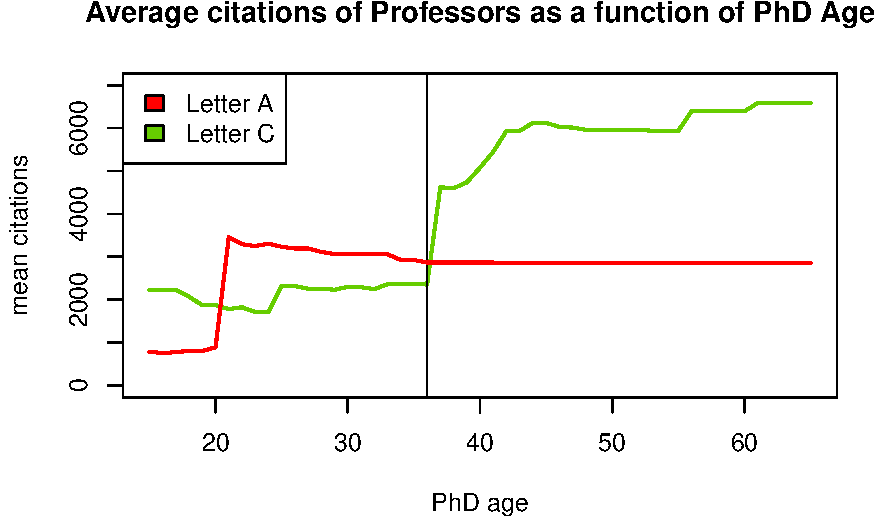
\includegraphics{index_files/figure-latex/unnamed-chunk-42-1.pdf}

The maximum age since PhD of a letter signer of A is 49. If he were to
cutoff his comparison at that point, clearly \(C>A\). If he were to
cutoff his comparison at 38, \(C>A\). Any further left of 36, he would
be accused of being biased.

Notice the spike at age 21. This is caused by Lior Pachter. What would
happen if we removed Pachter?

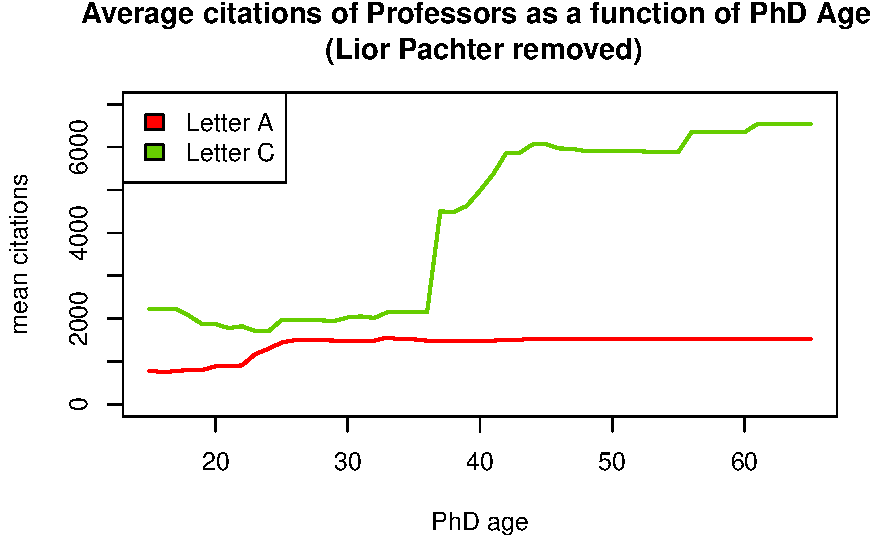
\includegraphics{index_files/figure-latex/unnamed-chunk-44-1.pdf}

So it is clear that Pachter's analysis was some sort of magic trick,
potentially a thought experiment, and a fraudulent one. It is highly
unlikely that a tenured and respected expert in computation and
statistics did not know the above result, expecially when a student he
suggests take an introductory statistics course immediately spotted it.
We claim and assert that he purposefully chose his 36 cutoff to try to
undermine our results.

\hypertarget{tier-rankings}{%
\subsection{Tier Rankings}\label{tier-rankings}}

In our excel sheet, (which we understand is the bane of
reproducibility), and through the magic of pivot tables, we rank R1
departments by calculating average department citations per year (since
first publication).

The top 11 departments using this ranking are:

\begin{enumerate}
\def\labelenumi{\arabic{enumi}.}
\item
  Princeton
\item
  Institute of Advanced Studies
\item
  Harvard
\item
  Stanford
\item
  University of Chicago
\item
  University of California - Los Angeles
\item
  Massachussetts Institute of Technology
\item
  Columbia University
\item
  New York University
\item
  University of Miami
\item
  University of California - Berkeley
\end{enumerate}

We calculate the average citations/average year since PhD of letters A,
B, and C, and compare them to our ranked list.

The average Math Sci Net Citations per year (PhD Age) is:

\begin{enumerate}
\def\labelenumi{\arabic{enumi}.}
\item
  For letter A - 15.98726
\item
  For letter B - 41.86467
\item
  For letter C - 55.3615
\end{enumerate}

Temple has an average citations per year of 12.33, so we retract our
claim that letter A is comparable to Temple. It is closer to the
University of Massachusetts - Amherst which has an average citations per
year of 16.17. By
\href{https://www.usnews.com/best-graduate-schools/top-science-schools/mathematics-rankings}{US
News}, University of Massachusetts - Amherst's Math Department has a
rank of 55. Rutgers has an average citations per year of 35.01, so we
retract our claim that letter B is comparable to Rutgers. It is closer
to the University of Minesotta which has an average citations per year
of 42.07 and a US News Ranking of 19. For Letter C, we claimed that it
was another tier higher - indeed it is closer to the University of
Chicago, which has an average citations per year of 56.27, ranked 6 by
US News.

An astute observer would notice we are not exactly comparing apples to
apples. Presumably ones first publication could be before one finishes
their PhD. So even with the boost, the order amongst letter signers
stands.

\hypertarget{discussion-and-conclusion}{%
\subsection{Discussion and Conclusion}\label{discussion-and-conclusion}}

We have debunked the claim that age is the greatest contributor for the
difference in citations and citations per year between signers of Letter
A, B, and C. Indeed, the least meritorious of mathematicians as a whole
signed letter A, whereas the more meritorious signed letters B and C,
with merit judged by citations. If one was not willing to believe
citations impose even a small order on merit, one could replace
citations with Fields medals, AMS Fellowships, or many other metrics.
One could make extrapolations by coupling this analysis with work by
Topaz, but we refrain from doing so.

In this analysis, we have addressed most of the criticisms in Pachter's
review, acknowledging our errors when pointed, while rejecting his false
claim that age was the greates confounder. The only one we have not
addressed is his point that, ``several p-values are computed and
reported without any multiple testing correction.'' After consultation
with a respected statistician, we do not see what the issue is. We
reported every p-value and he is welcome to change the set.seed in our
code, which he applauds us as easily reproducible.

Regarding the Russians, one cannot help but make parallels with what is
happening now in the USA with what happened in the USSR and China.
Mandatory diversity statements are being used as
\href{https://whyevolutionistrue.wordpress.com/2019/12/31/life-science-jobs-at-berkeley-with-hiring-giving-precedence-to-diversity-and-inclusion-statements/?fbclid=IwAR1tnpRsEfr43Y4b47EtScpSH_sUdhuqcfjBmi0Ez0uhxrK-aW4lR4C9sfg}{a
proxy for affirmative action}. Affirmative Action is wrong and is
totally pernicious. Advocates of affirmative action seem to believe
there is a tradeoff between ability and background, and that someone's
race, class, gender, sexual orientation, etc. is an excuse for bad
research. This is totally false. There are many strong female
mathematicians, there are many strong black mathematicians, there are
many strong gay mathematicians. There is nothing about someone's
background which can justify bad science.

Pachter ends his review by saying ``under-represented minorities and
women routinely face discrimination and worse. This is completely
unacceptable.'' We agree. But we do not believe that the solution is to
allow for more diverse faculty regardless of their ability as
researchers. What we do believe is that increasing opportunities for
under represented minorities at an early stage and fairer hiring
practices is the solution, not reverse discrimination
\href{https://blogs.ams.org/inclusionexclusion/2017/05/11/get-out-the-way/}{advocated
by some}.

We conclude by reiterating our thanks to Pachter. We truly appreciated
your review.

\hypertarget{data-and-code}{%
\subsection{Data and Code}\label{data-and-code}}

All code and data used for this report is available at.
\url{https://github.com/joshp112358/Response-to-Pachter}

\hypertarget{references}{%
\subsection{References}\label{references}}

Lior Pachter's Blog Post - Diversity Matters - January 17, 2020
\url{https://liorpachter.wordpress.com/2020/01/17/diversity-matters/}

Chad Topaz's Paper - Version 10 -
\url{https://osf.io/preprints/socarxiv/fa4zb/}

Our original Paper - Version 1 -
\url{https://arxiv.org/pdf/2001.00670.pdf}

In Preparation - A Citations Analysis of R1 Math Departments by Joshua
Paik and Igor Rivin

\hypertarget{miscellany}{%
\subsection{Miscellany}\label{miscellany}}

There seems to be some squabbles in the comments of Pachter's blog
whether the paper is Paik-Rivin or Rivin-Paik. In mathematics, we follow
the Hardy-Littlewood rule, namely all authors are first authors and we
list authors alphabetically.


\end{document}
